\chapter{Triggers}

\section{Trigger Properties}

The \menustyle{Setup / Trigger} menu opens the trigger properties dialog (Fig. \ref{trigger-properties}).

The Trigger Type box allows the type of trigger to be chosen. The list of available triggers depends on the instrument
model and installed software options.

The Trigger Offset field specifies the time from the \emph{start} of the waveform to the trigger point. Positive values
move the trigger later into the waveform, negative values introduce a delay between the trigger and the start of the
waveform. \footnote{This is a different convention than most oscilloscopes, which measure the trigger position from the
\emph{midpoint} of the waveform. Since glscopeclient decouples the acquisition length from the UI zoom setting,
measuring from the midpoint makes little sense as there are no obvious visual cues to the midpoint's location.}

\begin{figure}[h]
\centering
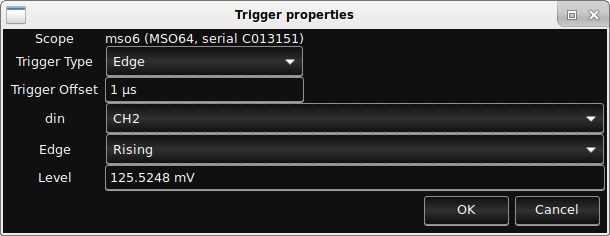
\includegraphics[width=9cm]{images/trigger-properties.png}
\caption{Trigger properties dialog}
\label{trigger-properties}
\end{figure}

The remaining settings in the trigger properties dialog depend on the specific trigger type chosen.

\section{Serial Pattern Triggers}

All serial pattern triggers take one or two pattern fields, a radix, and a condition.

For conditions like ``between" or ``not between" both patterns are used, and no wildcards are allowed. For other
conditions, only the first pattern is used.

Patterns may be specified as ASCII text, hex, or binary. ``Don't care" nibbles/bits may be specified in hex/binary
patterns as ``X", for example ``3fx8" or ``1100010xxx1".

\pagebreak

%%%%%%%%%%%%%%%%%%%%%%%%%%%%%%%%%%%%%%%%%%%%%%%%%%%%%%%%%%%%%%%%%%%%%%%%%%%%%%%%%%%%%%%%%%%%%%%%%%%%%%%%%%%%%%%%%%%%%%%%
\section{Dropout}

Triggers when a signal stops toggling for a specified amount of time.

\subsection{Inputs}

\begin{tabularx}{16cm}{llX}
\thickhline
\textbf{Signal name} & \textbf{Type} & \textbf{Description} \\
\thickhline
din & Analog or digital & Input signal \\
\end{tabularx}

\subsection{Parameters}

\begin{tabularx}{16cm}{llX}
\thickhline
\textbf{Parameter name} & \textbf{Type} & \textbf{Description} \\
\thickhline
Edge & Enum & Specifies the polarity of edge to look for (rising or falling) \\
\thickhline
Dropout Time & Int & Dropout time needed to trigger \\
\thickhline
Level & Float & Voltage threshold\\
\thickhline
Reset Mode & Enum & Specifies whether to reset the timer on the opposite edge \\
\thickhline
\end{tabularx}

%%%%%%%%%%%%%%%%%%%%%%%%%%%%%%%%%%%%%%%%%%%%%%%%%%%%%%%%%%%%%%%%%%%%%%%%%%%%%%%%%%%%%%%%%%%%%%%%%%%%%%%%%%%%%%%%%%%%%%%%
\section{Edge}

Triggers on edges in the signal.

Edge types ``rising" and ``falling" are self-explanatory. ``Any" triggers on either rising or falling edges.
``Alternating" is a unique trigger mode only found on certain Agilent/Keysight oscilloscopes, which alternates each
waveform between rising and falling edge triggers.

\subsection{Inputs}

\begin{tabularx}{16cm}{llX}
\thickhline
\textbf{Signal name} & \textbf{Type} & \textbf{Description} \\
\thickhline
din & Analog or digital & Input signal \\
\end{tabularx}

\subsection{Parameters}

\begin{tabularx}{16cm}{llX}
\thickhline
\textbf{Parameter name} & \textbf{Type} & \textbf{Description} \\
\thickhline
Edge & Enum & Specifies the polarity of edge to look for\\
\thickhline
Level & Float & Voltage threshold\\
\thickhline
\end{tabularx}

%%%%%%%%%%%%%%%%%%%%%%%%%%%%%%%%%%%%%%%%%%%%%%%%%%%%%%%%%%%%%%%%%%%%%%%%%%%%%%%%%%%%%%%%%%%%%%%%%%%%%%%%%%%%%%%%%%%%%%%%

\section{Pulse Width}

Triggers when a high or low pulse meeting specified width criteria is seen.

\begin{tabularx}{16cm}{llX}
\thickhline
\textbf{Signal name} & \textbf{Type} & \textbf{Description} \\
\thickhline
din & Analog or digital & Input signal \\
\end{tabularx}

\subsection{Parameters}

\begin{tabularx}{16cm}{llX}
\thickhline
\textbf{Parameter name} & \textbf{Type} & \textbf{Description} \\
\thickhline
Condition & Enum & Match condition (greater, less, between, or not between) \\
\thickhline
Edge & Enum & Specifies the polarity of edge to look for\\
\thickhline
Level & Float & Voltage threshold\\
\thickhline
Lower Bound & Int & Lower width threshold\\
\thickhline
Upper Bound & Int & Upper width threshold\\
\thickhline
\end{tabularx}

%%%%%%%%%%%%%%%%%%%%%%%%%%%%%%%%%%%%%%%%%%%%%%%%%%%%%%%%%%%%%%%%%%%%%%%%%%%%%%%%%%%%%%%%%%%%%%%%%%%%%%%%%%%%%%%%%%%%%%%%
\section{Runt}

Triggers when a pulse of specified width crosses one threshold, but not a second.

\begin{tabularx}{16cm}{llX}
\thickhline
\textbf{Signal name} & \textbf{Type} & \textbf{Description} \\
\thickhline
din & Analog & Input signal \\
\end{tabularx}

\subsection{Parameters}

\begin{tabularx}{16cm}{llX}
\thickhline
\textbf{Parameter name} & \textbf{Type} & \textbf{Description} \\
\thickhline
Condition & Enum & Match condition (greater, less, between, or not between) \\
\thickhline
Edge Slope & Enum & Specifies the polarity of edge to look for\\
\thickhline
Lower Interval & Int & Lower width threshold\\
\thickhline
Lower Level & Float & Lower voltage threshold\\
\thickhline
Upper Interval & Int & Upper width threshold\\
\thickhline
Upper Level & Float & Upper voltage threshold\\
\thickhline
\end{tabularx}

%%%%%%%%%%%%%%%%%%%%%%%%%%%%%%%%%%%%%%%%%%%%%%%%%%%%%%%%%%%%%%%%%%%%%%%%%%%%%%%%%%%%%%%%%%%%%%%%%%%%%%%%%%%%%%%%%%%%%%%%
\section{Slew Rate}

Triggers when an edge is faster or slower than a specified rate.

\begin{tabularx}{16cm}{llX}
\thickhline
\textbf{Signal name} & \textbf{Type} & \textbf{Description} \\
\thickhline
din & Analog & Input signal \\
\end{tabularx}

\subsection{Parameters}

\begin{tabularx}{16cm}{llX}
\thickhline
\textbf{Parameter name} & \textbf{Type} & \textbf{Description} \\
\thickhline
Condition & Enum & Match condition (greater, less, between, or not between) \\
\thickhline
Edge Slope & Enum & Specifies the polarity of edge to look for\\
\thickhline
Lower Interval & Int & Lower width threshold\\
\thickhline
Lower Level & Float & Lower voltage threshold\\
\thickhline
Upper Interval & Int & Upper width threshold\\
\thickhline
Upper Level & Float & Upper voltage threshold\\
\thickhline
\end{tabularx}

%%%%%%%%%%%%%%%%%%%%%%%%%%%%%%%%%%%%%%%%%%%%%%%%%%%%%%%%%%%%%%%%%%%%%%%%%%%%%%%%%%%%%%%%%%%%%%%%%%%%%%%%%%%%%%%%%%%%%%%%
\section{UART}

Triggers when a byte or byte sequence is seen on a UART.

\subsection{Inputs}

\begin{tabularx}{16cm}{llX}
\thickhline
\textbf{Signal name} & \textbf{Type} & \textbf{Description} \\
\thickhline
din & Analog or digital & Input signal \\
\end{tabularx}

\subsection{Parameters}

\begin{tabularx}{16cm}{llX}
\thickhline
\textbf{Parameter name} & \textbf{Type} & \textbf{Description} \\
\thickhline
Bit Rate & Int & Baud rate \\
\thickhline
Condition & Enum & Match condition \\
\thickhline
Level & Float & Voltage threshold\\
\thickhline
Parity Mode & Enum & Odd, even, or no parity \\
\thickhline
Pattern & String & First match pattern\\
\thickhline
Pattern 2 & String & Second match pattern \\
\thickhline
Polarity & Enum & Idle high (normal UART) or idle low (RS232)\\
\thickhline
Radix & Enum & Radix for the patterns\\
\thickhline
Stop Bits & Float & Number of stop bits\\
\thickhline
Trigger Type & Enum & Match data pattern or parity error\\
\thickhline
\end{tabularx}

%%%%%%%%%%%%%%%%%%%%%%%%%%%%%%%%%%%%%%%%%%%%%%%%%%%%%%%%%%%%%%%%%%%%%%%%%%%%%%%%%%%%%%%%%%%%%%%%%%%%%%%%%%%%%%%%%%%%%%%%

\section{Window}

Triggers when a signal goes above or below specified thresholds.

\begin{tabularx}{16cm}{llX}
\thickhline
\textbf{Signal name} & \textbf{Type} & \textbf{Description} \\
\thickhline
din & Analog & Input signal \\
\end{tabularx}

\subsection{Parameters}

\begin{tabularx}{16cm}{llX}
\thickhline
\textbf{Parameter name} & \textbf{Type} & \textbf{Description} \\
\thickhline
Lower Level & Float & Lower voltage threshold\\
\thickhline
Upper Level & Float & Upper voltage threshold\\
\thickhline
\end{tabularx}

